\documentclass[t]{beamer}

\usetheme{TU}

\hypersetup{unicode=true,pdfcreator={},pdfproducer={}}

\usepackage{booktabs}
\usepackage{array}
\usepackage{setspace}
\usepackage{minted}
\usepackage{textcmds}

\title{Toolbox Workshop}
\subtitle{Nützliche Programme für Physikstudenten}
\author[Igor B.\and Kevin D.\and Christian G.\and Peter L.\and Ismo T.]{
       Igor Babuschkin%\thanks{\href{mailto:igor.babuschkin@udo.edu}{igor.babuschkin@udo.edu}}
  \and Kevin Dungs%\thanks{\href{mailto:kevin.dungs@udo.edu}{kevin.dungs@udo.edu}}
  \and Christian Gerhorst%\thanks{\href{mailto:christiangerhorst@gmail.com}{christiangerhorst@gmail.com}}
  \and Peter Lorenz%\thanks{\href{mailto:peter.lorenz@udo.edu}{peter.lorenz@udo.edu}}
  \and Ismo Toijala%\thanks{\href{mailto:ismo.toijala@udo.edu}{ismo.toijala@udo.edu}}
}
\institute[PeP et al. e.V.]{
  PeP et al. e.V.%\thanks{\href{http://pep-dortmund.org}{pep-dortmund.org}}
}
\date{September 2012}

\begin{document}
\begin{frame}
  \begin{center}
    
\includegraphics[width=.5\paperwidth]{logos/pep.pdf} \\
    \color{TUgreen}\textbf{\href{http://pep-dortmund.org}{www.pep-dortmund.org}}
  \end{center}
  \begin{itemize}
    \item Einrichtung für Absolventen, Studierende, Mitarbeiter sowie Freunde und Förderer der Fakultät Physik
    \item Mission: Netzwerk zwischen Absolventen und der Fakultät aufbauen
  \end{itemize}
\end{frame}

\begin{frame}{Motivation}
  \begin{itemize}
    \item Arbeitserleichterung
    \item ``Gute'' Tools \begin{itemize}
      \item Kein Excel!
    \end{itemize}
  \item Teamarbeit++
  \item \textit{best practices}
  \end{itemize}  
\end{frame}

\chapter{Python}
\begin{center}
  
\includegraphics[width=140px]{img/python.png} \\
  \textbf{\url{http://python.org}}
\end{center}
\begin{quote}
  \textit{Python is a programming language that lets you work more quickly and integrate your systems more effectively.
          You can learn to use Python and see almost immediate gains in productivity and lower maintenance costs.}
\end{quote}

\section{IPython}
Python selbst kommt mit einer interaktiven Kommandozeile (genauer: einer REPL\footnote{read–eval–print loop}-Umgebung).
Um einen Einblick in die Sprache zu erhalten, ist diese eigentlich vollkommen ausreichend.
Sie bietet die Möglichkeit, interaktiv mit der Sprache in Kontakt zu kommen.
IPython erlaubt zusätzlich, auf die Shell zuzugreifen und interaktive Sitzungen zu speichern.
Gestartet wird IPython auf der Kommandozeile mit
\begin{verbatim}
ipython3
\end{verbatim}
und meldet sich (zum Beispiel hier unter OS X mit Python 3.2.3) mit der Ausgabe
\begin{verbatim}
Python 3.2.3 (default, Apr 13 2012, 00:15:25) 
Type "copyright", "credits" or "license" for more information.

IPython 0.13 -- An enhanced Interactive Python.
?         -> Introduction and overview of IPython's features.
%quickref -> Quick reference.
help      -> Python's own help system.
object?   -> Details about 'object', use 'object??' for extra details.

In [1]: 
\end{verbatim}
Um IPython zu beenden gibt es die Befehle \texttt{exit}, \texttt{exit()}, \texttt{quit}, \texttt{quit()} und natürlich \texttt{Ctrl-D}.

\section{Syntax}
Grundsätzlich ist die Python-Syntax sehr einfach und intuitiv.
In vielen Punkten erinnert sie eher an eine Scriptsprache.

\paragraph{Blöcke}
Durch Einrückung!
4 Leerzeichen (/1 Tab)

\paragraph{Semikolons}
Gibt es prinzipiell
Sind am Zeilenende aber nicht notwendig

\paragraph{???}
In einer interaktiven Sitzung (z.B. IPython) können zum Einstieg einfache mathematische Berechnungen durchgeführt werden:
\begin{verbatim}
In [1]: 1 + 2
Out[1]: 3

In [2]: 1 * 2
Out[2]: 2
\end{verbatim}

\subsection{Variablen}
Natürlich gibt es Variablen.
Dynamische Typisierung
Keine explizite Deklaration 
Ihre Verwendung ist denkbar einfach:
\begin{verbatim}
In [3]: a = 2

In [4]: a
Out[4]: 2

In [5]: b = 1 + 1

In [6]: b
Out[6]: 2
\end{verbatim}
Variablennamen können Buchstaben, Zahlen und Unterstrichte enthalten, dürfen jedoch nicht mit einer Ziffer beginnen.

\subsection{Datenstrukturen/-typen}
\begin{itemize}
  \item bool (\texttt{True}, \texttt{False})
  \item int, float, long, complex
  \item string (\texttt{'foo'}, \texttt{"bar"})
  \item Iteratoren, Generatoren, Sequenzen, …
\end{itemize}
\paragraph{Praktische Typen}
\begin{itemize}
  \item[\texttt{()}] Tupel
  \item[\texttt{[]}] Liste
  \item[\texttt{\{\}}] Dictionary 
\end{itemize}
\paragraph{Zum Beispiel}
\begin{minted}{python}
In [9]: cities = ['Dortmund', 'Hamburg', 'Berlin']

In [10]: cities[0]
Out[10]: 'Dortmund'
\end{minted}
\paragraph{Mehr Beispiele}
\begin{minted}{python}
In [1]: teams = {
   ...:         'BVB': "BV Borussia Dortmund 09",
   ...:         'S04': "FC Schalke 04",
   ...:         'FCB': "FC Bayern München"
   ...: }

In [2]: teams['BVB']
Out[2]: 'BV Borussia Dortmund 09'
\end{minted}


\subsection{Operatoren}
Wie aus dem obigen Beispiel hervorgeht, gibt es in Python \textbf{mathematische Operatoren}.
In \autoref{tab:op_mat} sind diese dargestellt.

\begin{table}[H]
  \centering{}
  \caption{Mathematische Operatoren}
  \label{tab:op_mat}
  \begin{tabular}{c l c c}
    \toprule
    Op.         & Funktion         & Beispiel         & Ergebnis \\
    \midrule
    \texttt{+}  & Addition         & \texttt{1 + 2}   & \texttt{3} \\
    \texttt{-}  & Subtraktion      & \texttt{1 - 2}   & \texttt{-1} \\
    \texttt{*}  & Multiplikation   & \texttt{1 * 2}   & \texttt{2} \\
    \texttt{/}  & Division         & \texttt{1 / 2}   & \texttt{0.5} \\
    \texttt{\%} & Modulo           & \texttt{11 \% 2} & \texttt{1} \\
    \texttt{**} & Exponent         & \texttt{2**3}  & \texttt{8} \\
    \texttt{//} & Ganzzahldivision & \texttt{5 // 2}  & \texttt{2} \\
    \bottomrule
  \end{tabular}
\end{table}

\textbf{Zuweisungsoperatoren} setzen sich aus einem mathematischen Operator und einem Gleichheitszeichen zusammen.
Mit ihnen kann gleichzeitig eine Berechnung und eine Zuweisung durchgeführt werden, zum Beispiel:
\begin{verbatim}
In [7]: a = 2

In [7]: a *= 3

In [8]: a
Out[8]: 6
\end{verbatim}

Mit Hilfe von \textbf{Vergleichsoperatoren} (siehe \autoref{tab:op_comp}) lassen sich Vergleiche durchführen.
\begin{table}[H]
  \centering{}
  \caption{Vergleichsoperatoren}
  \label{tab:op_comp}
  \begin{tabular}{c l c c}
    \toprule
    Op.             & Funktion            & Beispiel        & Ergebnis \\
    \midrule
    \texttt{==}     & Gleich              & \texttt{1 == 1} & \texttt{True} \\
    \texttt{!=}     & Ungleich            & \texttt{2 != 1} & \texttt{True} \\
    \texttt{>}      & Größer              & \texttt{2 > 1}  & \texttt{True} \\
    \texttt{<}      & Kleiner             & \texttt{1 < 2}  & \texttt{True} \\
    \texttt{>=}     & Größer oder gleich  & \texttt{2 >= 1} & \texttt{True} \\
    \texttt{<=}     & Kleiner oder gleich & \texttt{1 <= 2} & \texttt{True} \\
    \bottomrule
  \end{tabular}
\end{table}

\paragraph{Logische Operatoren}
\begin{minted}{python}
and, or, not
\end{minted}
\paragraph{Identitätsoperatoren}
\begin{minted}{python}
is, is not
\end{minted}
\paragraph{Operatoren für Sequenzen}
\begin{minted}{python}
in, not in
\end{minted}

\subsection{Dateien} 
python
    open
    file
        write
    range
    len
    string
        format
        join
    list
        append
        index
    dict
    sorted
    decimal
    math
        floor
        ceil
    convert
        str
        int
        float

\section{Bibliotheken}
\subsection{NumPy}
NumPy ist eine Bibliothek für Python, die diverse Features unterstützt, die wissenschaftliches Arbeiten deutlich erleichtern.
Einige davon sind
\begin{itemize}
  \item ein $n$-dimensionales Array-Objekt
  \item ausgeklügelte, durchdachte Funktionen für Optimierung, Integration und Interpolation
  \item die Möglichkeit C/C++- und Fortran-Code zu integrieren
  \item Tools für Lineare Algebra, Fouriertransformation, Statistik
  \item beliebige eigene Datentypen können definiert werden
\end{itemize}

\subsection{SciPy}
SciPy ist, ähnlich wie NumPy, eine Bibliothek, die wissenschaftliches Arbeiten erleichtert.
Insbesondere sind in dem Paket verschiedene Konstanten gespeichert, die im Praktikum oft gebraucht werden.
SciPy ist eine Erweiterung von NumPy, die vor allem vom NumPy-Array profitiert.
Es besitzt ebenfalls viele benutzerfreundliche und effiziente numerische Algorithmen für Integration und Optimierung.

\subsection{matplotlib}
Bei matplotlib handelt es ich um eine Bibliothek für Plots.
\begin{quote}
  \textit{matplotlib tries to make easy things easy and hard things possible.}
\end{quote}
Es dient dazu Plots, auch polare, sowie Fehlerbalken und noch vieles mehr zu Plotten.
Es bietet sehr viele Einstellungsmöglichkeiten mit denen man den Plot anpassen kann.
matplotlib bietet eine objektorientierte API, die erlaubt die Plots in Anwendungen einzubetten die generische GUI-Toolkits wie Qt oder GTK benutzen.
Es gibt ebenfalls PyLab, das die verwendung in IPython erleichtert.

\subsubsection{Objektorientiertes Interface}
\begin{figure}[H]
  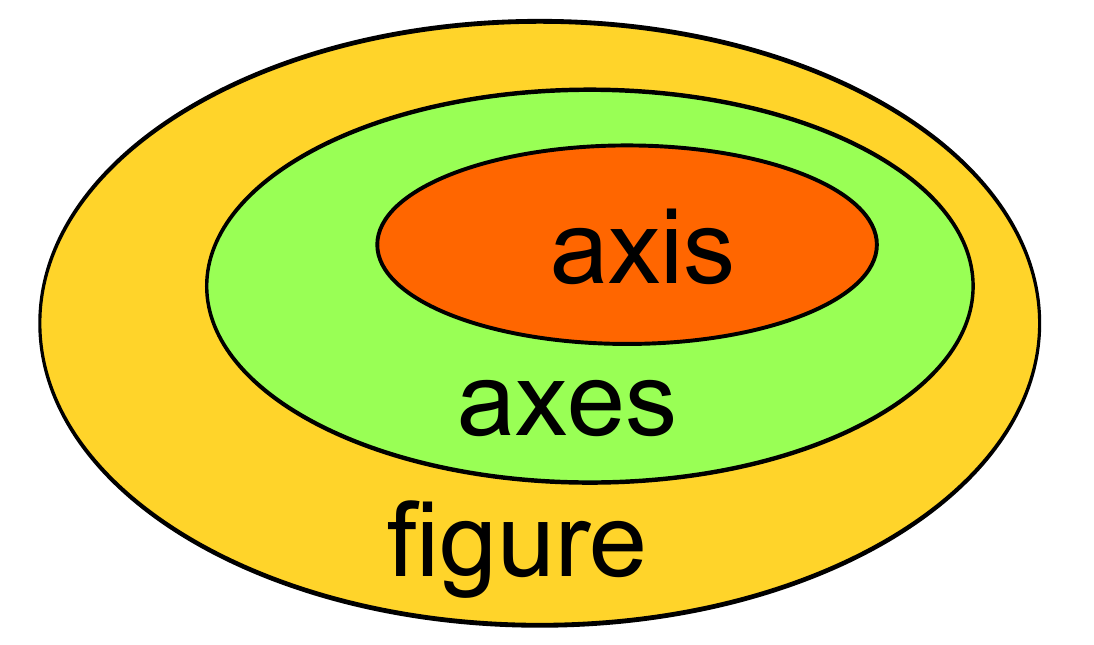
\includegraphics[width=150px]{img/matplotlib_v.png}
\end{figure}
\begin{itemize}
  \item figure: Leinwand, auf die Plots projiziert werden
  \item axes: enthält Plot, der beliebig in der figure plaziert werden kann
  \item axis: Koordinatenachsen 
\end{itemize}

\subsubsection{Linienstyles und Farben}
Die Übersichten in \autoref{tab:plt_lines} und \autoref{tab:plt_colors} stammen von \url{http://www.thetechrepo.com/main-articles/469-how-to-change-line-properties-in-matplotlib-python}.

\begin{table}[H]
  \centering{}
  \caption{Linienstile}
  \label{tab:plt_lines}
  \begin{tabular}{c l}
    \toprule
      Buchstabe & Stil \\
    \midrule
      \texttt{-} & solid line style \\
      \texttt{--} & dashed line style \\
      \texttt{-}. &  dash-dot line style \\
      \texttt{:} & dotted line style \\
      \texttt{.} & point marker \\
      \texttt{,} & pixel marker \\
      \texttt{o} & circle marker \\
      \texttt{v} & triangle\_down marker \\
      \texttt{\^{}} & triangle\_up marker \\
      \texttt{<} & triangle\_left marker \\
      \texttt{>} & triangle\_right marker \\
      \texttt{1} & tri\_down marker \\
      \texttt{2} & tri\_up marker \\
      \texttt{3} & tri\_left marker \\
      \texttt{4} & tri\_right marker \\
      \texttt{s} & square marker \\
      \texttt{p} & pentagon marker \\
      \texttt{*} & star marker \\
      \texttt{h} & hexagon1 marker \\
      \texttt{H} & hexagon2 marker \\
      \texttt{+} & plus marker \\
      \texttt{x} & x marker \\
      \texttt{D} & diamond marker \\
      \texttt{d} & thin\_diamond marker \\
      \texttt{|} & vline marker \\
      \texttt{\_} & hline marker \\
    \bottomrule
  \end{tabular}
\end{table}

\begin{table}[H]
  \centering{}
  \caption{Farben}
  \label{tab:plt_colors}
  \begin{tabular}{c l}
    \toprule
      Buchstabe & Farbe \\
    \midrule
      \texttt{k} & schwarz \\
      \texttt{w} & weiß \\
      \texttt{r} & rot \\
      \texttt{g} & grün \\
      \texttt{b} & blau \\
      \texttt{c} & cyan \\
      \texttt{y} & gelb \\
      \texttt{m} & magenta \\
    \bottomrule
  \end{tabular}
\end{table}


\section{Python 2}
Falls man Python 2 verwendet, sollte jede \texttt{.py}-Datei so anfangen:
\begin{verbatim}
# coding=utf-8
from __future__ import division, print_function, unicode_literals
\end{verbatim}
Dann funktionieren Division, \texttt{print} und Unicode wie in Python 3.
Man sollte dann auch immer \texttt{python2} und \texttt{ipython2} aufrufen.

\section{Weiterführende Links}
\begin{itemize}
  \item Learn Python The Hard Way (Python 2): \url{http://learnpythonthehardway.org/}
  \item Dive Into Python 3: \url{http://www.diveintopython3.net/}
  \item Python v3 documentation: \url{http://docs.python.org/py3k/}
  \item PEP 8 -- Style Guide for Python Code: \url{http://www.python.org/dev/peps/pep-0008/}
  \item Tentative NumPy Tutorial: \url{http://www.scipy.org/Tentative\_NumPy\_Tutorial}
  \item NumPy and SciPy Documentation: \url{http://docs.scipy.org/doc/}
  \item matplotlib Documentation: \url{http://matplotlib.org/1.2.0/contents.html}
  \item matplotlib Gallery: \url{http://matplotlib.org/1.2.0/gallery.html}
  \item Python Uncertainties package: \url{http://packages.python.org/uncertainties/}
  \item SymPy: \url{http://sympy.org/en/index.html}
  \item matplotlib tutorial: \url{http://www.loria.fr/~rougier/teaching/matplotlib/}
  \item Python Scientific Lecture Notes: \url{http://scipy-lectures.github.com/}
  \item PyCon 2012: \url{http://pyvideo.org/category/17/pycon-us-2012}
    \begin{itemize}
      \item Plotting with matplotlib: \url{http://pyvideo.org/video/617/plotting-with-matplotlib}
      \item IPython: Python at your fingertips: \url{http://pyvideo.org/video/640/ipython-python-at-your-fingertips}
      \item IPython in-depth: high-productivity interactive and parallel python: \url{http://pyvideo.org/video/605/ipython-in-depth-high-productivity-interactive-a}
      \item Python for data lovers: explore it, analyze it, map it: \url{http://pyvideo.org/video/676/python-for-data-lovers-explore-it-analyze-it-m}
      \item Sage: Open Source Math in Python: \url{http://pyvideo.org/video/652/sage-open-source-math-in-python}
    \end{itemize}
  \item SciPy 2012: \url{http://pyvideo.org/category/20/scipy\_2012}
    \begin{itemize}
      \item Introduction to NumPy and matplotlib: \url{http://pyvideo.org/video/1190/introduction-to-numpy-and-matplotlib}
      \item Advanced matplotlib: \url{http://pyvideo.org/video/1344/advanced-matplotlib}
      \item IPython: tools for the entire lifecycle of research computing: \url{http://pyvideo.org/video/1221/ipython-tools-for-the-entire-lifecycle-of-resear}
      \item A tale of four libraries: \url{http://pyvideo.org/video/1211/a-tale-of-four-libraries}
    \end{itemize}
  \item SciPy 2011: \url{http://archive.org/search.php?query=subject\%3A\%22SciPy2011\%22}
  \item Protokolle (manchmal nicht sehr schön…)
    \begin{itemize}
      \item Python-Bibliotheken, \LaTeX-Header: \url{https://bitbucket.org/ibab/powertools}
      \item Christian, Ismo (2011): \url{https://bitbucket.org/itoijala/ap-protokolle11}
      \item Christian, Ismo (2012): \url{https://bitbucket.org/itoijala/ap-protokolle12}
    \end{itemize}
\end{itemize}


\subsection{Bibliotheken}

\begin{frame}{Beispiele und Aufgaben herunterladen}
  Lade das Repository \\
  \url{https://github.com/ibab/toolbox} \\
  per \texttt{git clone} herunter.
\end{frame}

\subsubsection{PyLab}
\begin{frame}{PyLab}
  \begin{itemize}
    \item bündelt NumPy, SciPy und Matplotlib
    \item starten mit \texttt{ipython3 --pylab}
  \end{itemize}
\end{frame}

\subsubsection{NumPy}
\begin{frame}{NumPy}
  \begin{center}
    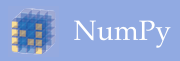
\includegraphics[width=100px]{../Notes/img/numpy.png}
  \end{center}
  \begin{itemize}
    \item $n$-dimensionale Arrays
    \item Funktionen, die auf denen arbeiten
    \item Operatoren wirken elementweise
    \item wird meist mit \texttt{np} abgekürzt
  \end{itemize}

  Konstanten:
  \begin{itemize}
    \item \texttt{pi}
    \item \texttt{e}
  \end{itemize}
\end{frame}

\begin{frame}{Arrays erstellen}
  \begin{itemize}
    \item \texttt{array}: konvertiert irgendwas (Liste, Tupel, …) zu einem Array
    \item \texttt{linspace(start, end, number)}: Array aus \texttt{number} Zahlen zwischen \texttt{start} und \texttt{end} in gleichem Abstand
    \item \texttt{arange(start, end, step)}: Array aus Zahlen zwischen \texttt{start} und \texttt{end} mit dem Abstand \texttt{step}
    \item \texttt{zeros(shape)}: Array aus Nullen der Größe \texttt{shape}
    \item \texttt{ones(shape)}: Array aus Einsen der Größe \texttt{shape}
  \end{itemize}
\end{frame}

\begin{frame}{Elementweise Funktionen}
  Beispiele:
  \begin{itemize}
    \item \texttt{sqrt}
    \item \texttt{exp}, \texttt{log}
    \item \texttt{sin}
    \item \texttt{deg2rad}, \texttt{rad2deg}
  \end{itemize}
\end{frame}

\begin{frame}{Reduzierende Funktionen}
  Beispiele:
  \begin{itemize}
    \item \texttt{sum}
    \item \texttt{mean}
    \item \texttt{max}, \texttt{min}
    \item \texttt{ediff1d}
  \end{itemize}
\end{frame}

\begin{frame}{It/Output}
  \begin{itemize}
    \item \texttt{loadtxt(file [, unpack=True])}: Lädt eine Datei in ein Array.
      \texttt{unpack=True} transponiert das Array
    \item \texttt{savetxt(file, array)}: Speichert ein Array in eine Datei
  \end{itemize}
\end{frame}

\subsubsection{SciPy}
\begin{frame}{SciPy}
  \begin{center}
    
\includegraphics{../Notes/img/scipy.pdf}
  \end{center}
\end{frame}

\begin{frame}{Nützliche Funktionen}
  \begin{itemize}
    \item \texttt{optimize.curve\_fit}: fittet nichtlineare Funktionen
    \item \texttt{stats.sem}: gibt den Fehler des Mittelwerts
    \item \texttt{constants.C2K}: konvertiert Celsius in Kelvin
    \item \texttt{constants.K2C}: konvertiert Kelvin in Celsius
  \end{itemize}
\end{frame}

\begin{frame}{Konstanten}
  \begin{itemize}
    \item \texttt{constants.physical\_constants}: enthält diverse physikalische Konstanten, ihre Fehler und Einheiten (aus CODATA)
  \end{itemize}
\end{frame}

\subsubsection{matplotlib}
\begin{frame}{matplotlib}
  \begin{center}
    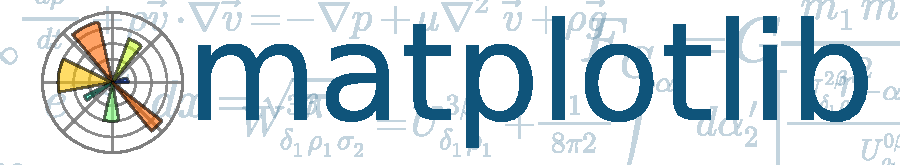
\includegraphics[width=\textwidth]{../Notes/img/matplotlib.pdf}
  \end{center}
  \begin{itemize}
    \item prozedurales Interface (pyplot, in PyLab) \mdash\ einfacher
    \item objektorientiertes Interface (Beschreibung im Skript) \mdash\ flexibler, schöner für größere Skripte oder Programme
  \end{itemize}
\end{frame}

\begin{frame}{Beispiele}
  \begin{center}
    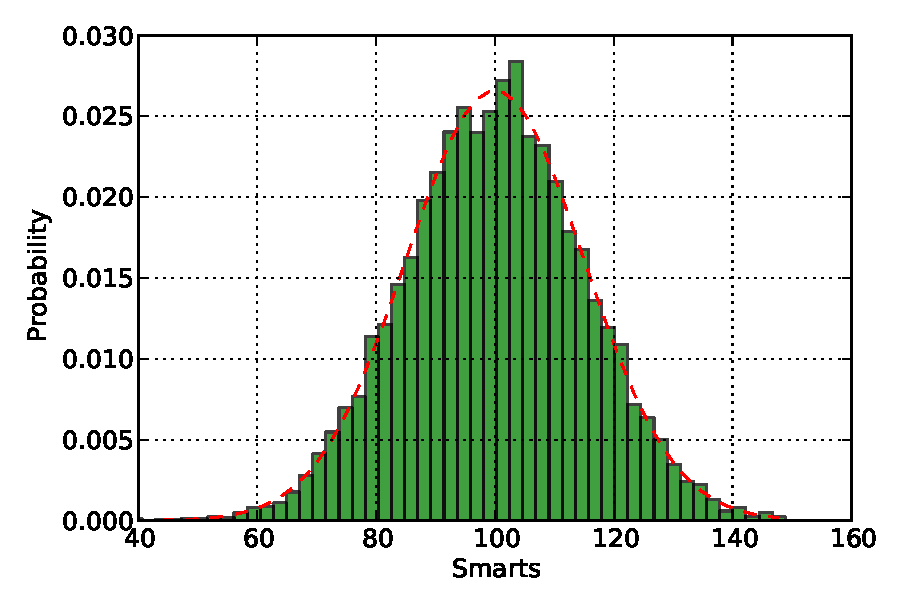
\includegraphics[width=0.8\textwidth]{img/matplotlib/hist.pdf}
  \end{center}
\end{frame}

\begin{frame}{Beispiele}
  \begin{center}
    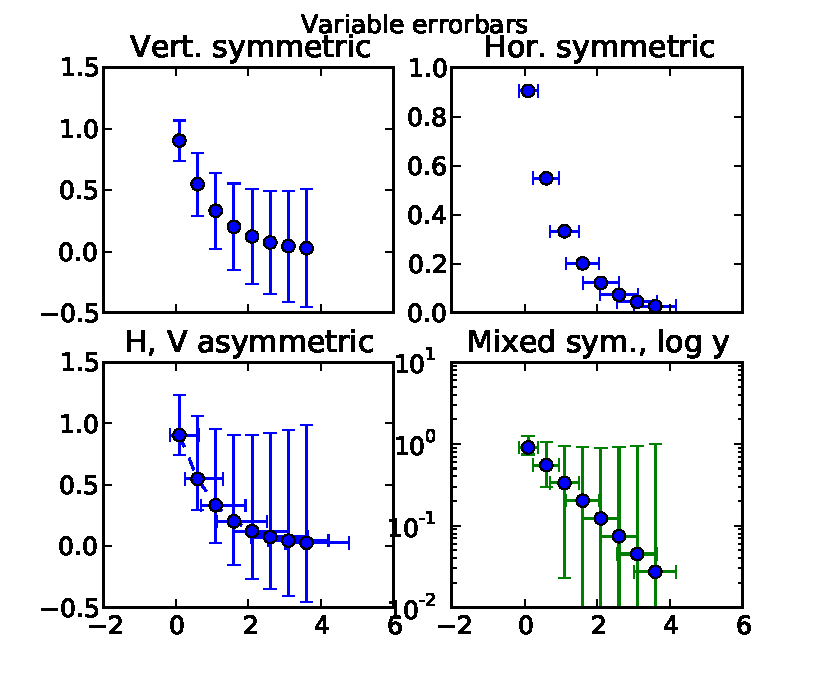
\includegraphics[width=0.8\textwidth]{img/matplotlib/errorbars.pdf}
  \end{center}
\end{frame}

\begin{frame}{Beispiele}
  \begin{center}
    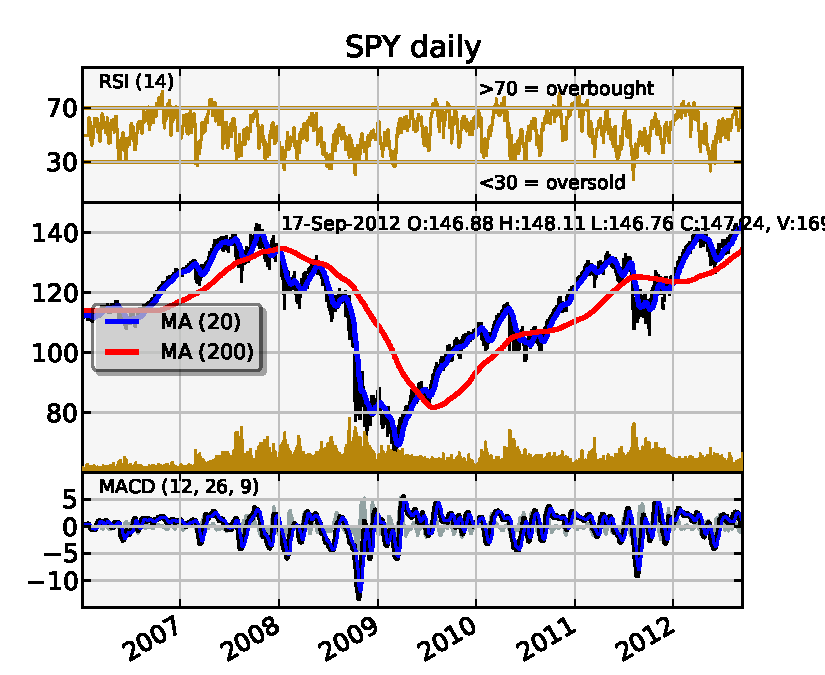
\includegraphics[width=0.8\textwidth]{img/matplotlib/finance.pdf}
  \end{center}
\end{frame}

\begin{frame}{Beispiele}
  \begin{center}
    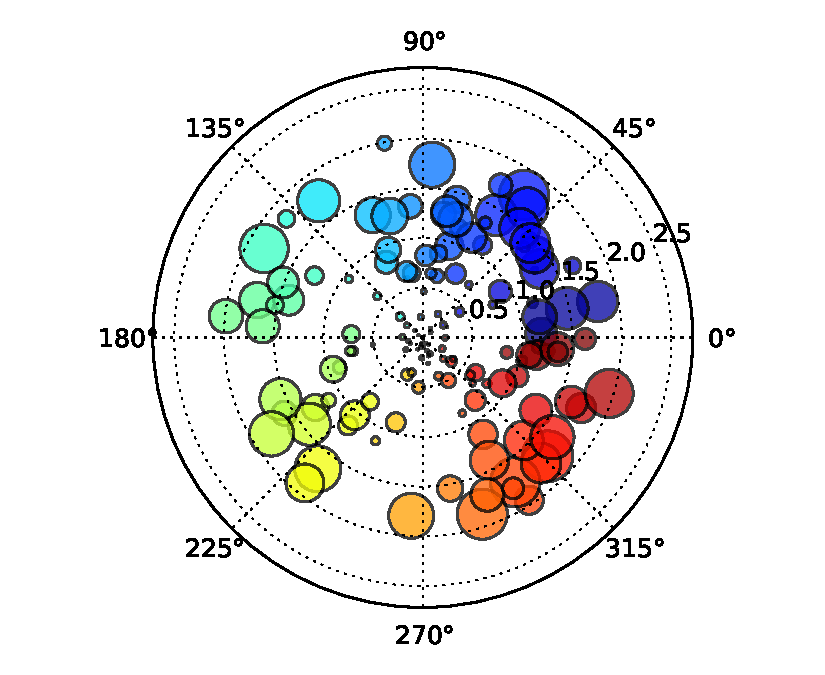
\includegraphics[width=0.8\textwidth]{img/matplotlib/polar.pdf}
  \end{center}
\end{frame}

\begin{frame}{Beispiele}
  \begin{center}
    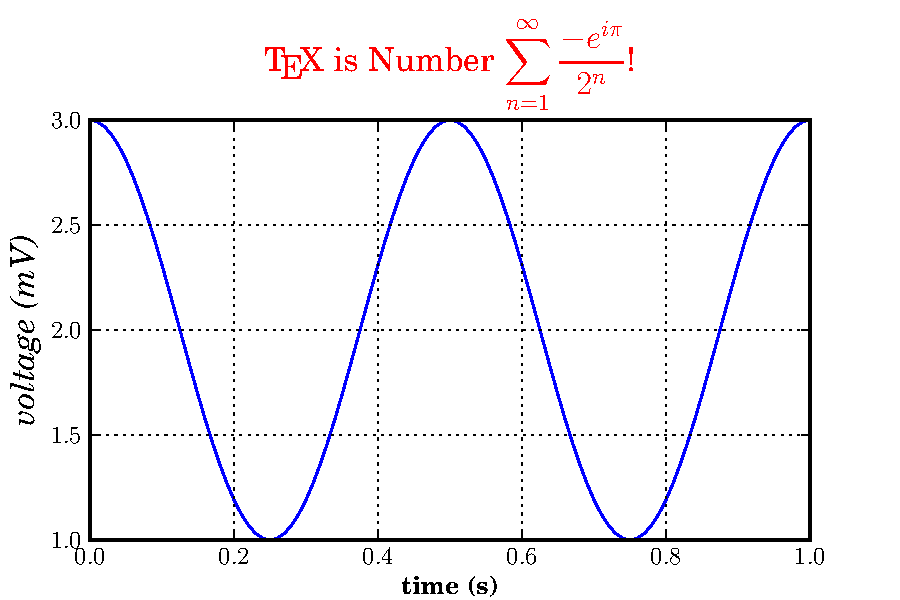
\includegraphics[width=0.8\textwidth]{img/matplotlib/tex.pdf}
  \end{center}
\end{frame}

\begin{frame}{Beispiele}
  \begin{center}
    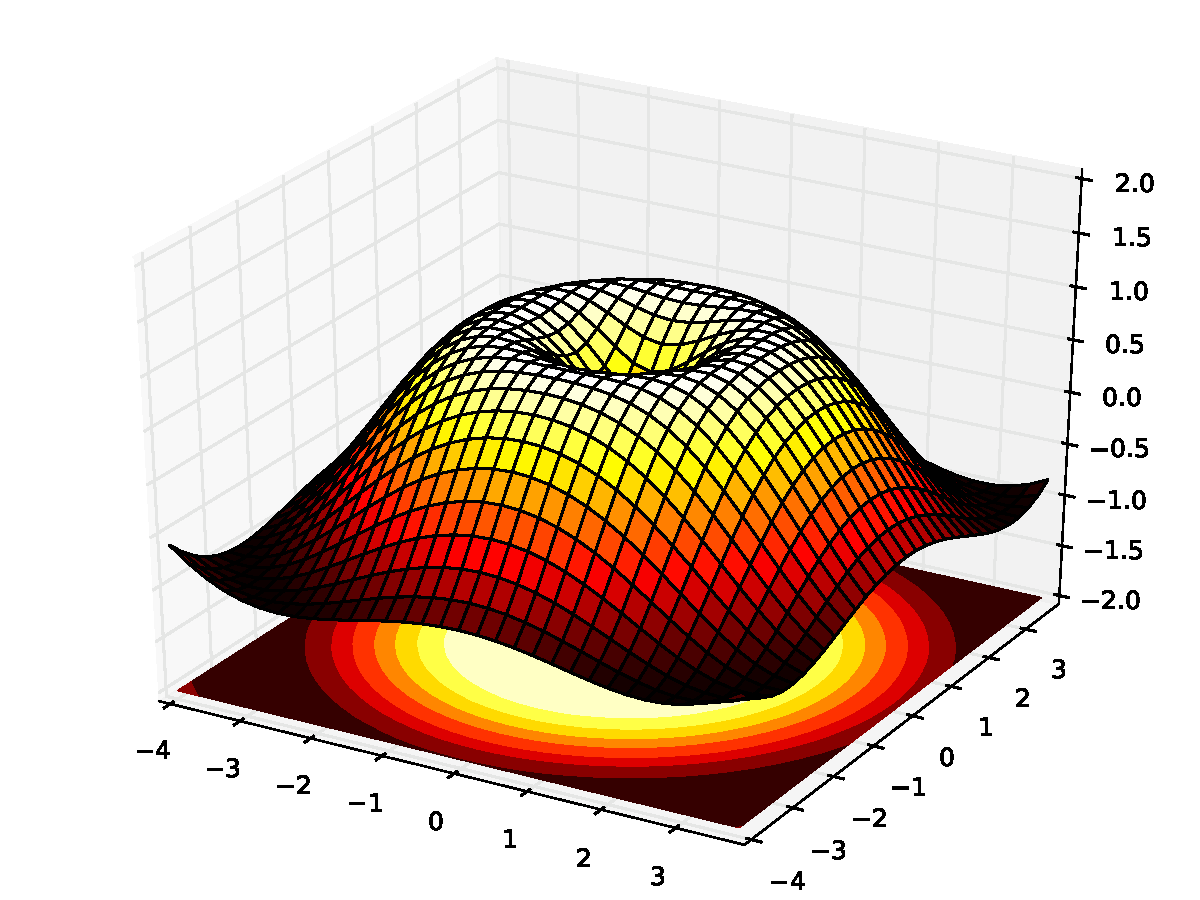
\includegraphics[width=0.8\textwidth]{img/matplotlib/mplot3d.pdf}
  \end{center}
\end{frame}

\begin{frame}[fragile]{Plotten mit IPython}
  Einfach \texttt{ipython3 --pylab} ausführen und z.B. Folgendes eintippen:
\begin{minted}{python}
  In [1]: x = linspace(0, 1, 100)
  In [2]: plot(x, x**2, 'b-')
\end{minted}
  An dem Plot kann interaktiv weiter gearbeitet werden.
\end{frame}

\begin{frame}[fragile]{Plots in .py-Dateien erstellen}
  Erst einmal Bibliotheken importieren.\\
  Plot erscheint, wenn man \texttt{show()} aufruft.
\begin{minted}{python}
from numpy import linspace, pi, sin
import matplotlib.pyplot as plt
x = linspace(0, 2 * pi, 1000)
plt.plot(x, sin(x), 'r--')
plt.show()
# oder: plt.savefig('plot.pdf')
\end{minted}
\end{frame}

\begin{frame}{Verschiedene Arten von Plots}
  \begin{itemize}
    \item \texttt{plot}
    \item \texttt{errorbar} - Plot mit Fehlerbalken
    \item \texttt{semilogy}, \texttt{semilogx} - logarithmische Skalierung
    \item \texttt{hist} - Histogramme
    \item \texttt{polar} - polare Plots
  \end{itemize}
\end{frame}

\begin{frame}{Nützliche Funktionen}
  \begin{itemize}
    \item \texttt{title('...')}
    \item \texttt{xlabel('...'), ylabel('...')}
    \item \texttt{grid()}
    \item \texttt{xlim(a, b)}, \texttt{ylim(a, b)}
    \item \texttt{legend()} (beim Plot \texttt{label='...'} einstellen
    \item \texttt{clf()}
  \end{itemize}
\end{frame}

\begin{frame}{Matplotlib einstellen}
  2 Möglichkeiten:
  \begin{itemize}
    \item direkt in der Code-Datei
    \item Datei \texttt{matplotlibrc} im selben Ordner
  \end{itemize}
  $\Rightarrow$ siehe Dokumentation
\end{frame}

\chapter{Unix Shell}
\begin{center}
    
\includegraphics[width=120px]{img/term.pdf} \\
    \textbf{\href{http://en.wikipedia.org/wiki/Unix_shell}{Unix Shell}}
\end{center}

\section{Dateisystem}
Das Dateisystem in Linux besteht aus \emph{einem} Baum.
Dies äußert sich im so genannten Dateipfad, der den Weg von der Wurzel \texttt{/} zur eigentlichen Datei oder dem Ordner beschreibt.
Nach jedem Knoten, das heißt nach jedem Überordner setzt man wieder ein Slash bis man beim Dateinamen angekommen ist.

Es gibt immer ein aktuelles Verzeichnis, in dem man sich befindet; dieses wird 'working directory' genannt.
Will man aus dem working directory in ein anderes Verzeichnis so kann man dies durch eine relative oder absolute Pfadangabe tuen.
Bei einem absoluten Pfad geht man wieder von der Wurzel aus und beginnt ihn mit \texttt{/}.
Wählt man den relativen Pfad, der oft kürzer ist, insbesondere wenn man einfach nur in den Über- oder Unterordner möchte, so baut man die Pfadangabe ausgehend vom aktuellen Verzeichnis auf.
Bei der Pfadangabe sollte man im Übrigen folgende besondere Verzeichnisse kennen:
    \begin{itemize}
      \item \texttt{.} das aktuelle Verzeichnis (oder der aktuelle im bisherigen Pfad, \texttt{a/./}~=~\texttt{a/})
      \item \texttt{..} das Oberverzeichnis des aktuellen Verzeichnisses (\texttt{a/b/../}~=~\texttt{a/})
      \item \texttt{\textasciitilde} das Heimverzeichnis (nur am Anfang eines Pfads)
    \end{itemize}

\section{Aufbau einer Eingabe}
\texttt{\$ ls -l --all \textit{directory}\\
        \textit{output}\\
        \$}
\begin{center}
  \begin{tabular}{>{\tt}l l}
    \toprule
    \$                 & Prompt       \\
    ls                 & Befehl       \\
    -l                 & kurze Option \\
    --all              & lange Option \\
    \textit{directory} & Argument     \\
    \textit{output}    & Ausgabe      \\
    \bottomrule
  \end{tabular}
\end{center}
\begin{itemize}
  \item \texttt{\$} ist nur ein Beispiel für einen Prompt, häufig wird das aktuelle Verzeichnis und/oder andere Informationen angezeigt
  \item kurze Optionen können zusammengefasst werden (\texttt{ls~-la} = \texttt{ls -l -a} = \texttt{ls -l --all})
  \item die Reihenfolge der Optionen ist egal
  \item meistens werden mehrere Argumente (z.B. Dateien) akzeptiert
\end{itemize}

\section{Befehle}
\subsection{\texttt{man}}
\begin{itemize}
  \item \texttt{man \textit{topic}} für manual: zeigt die Hilfe für ein Programm
  \item Beispiel: \texttt{man man}
\end{itemize}

\subsection{\texttt{pwd}, \texttt{cd}}
\begin{itemize}
  \item \texttt{pwd} für print working directory: zeigt das aktuelle Verzeichnis
  \item \texttt{cd \textit{directory}} für change directory: wechselt in das angegebene Verzeichnis
  \item Beispiel:
\begin{verbatim}
$ pwd
/home/ismo
$ cd ../../etc
$ pwd
/etc
$ cd ~
$ pwd
/home/ismo
\end{verbatim}
\end{itemize}

\subsection{ls}
\begin{itemize}
  \item \texttt{ls [\textit{directory}]} für list: zeigt den Inhalt eines Verzeichnisses an
  \item \texttt{ls -l}: zeigt mehr Informationen über Dateien und Verzeichnisse
  \item \texttt{ls -a}: zeigt auch versteckte Dateien
  \item \texttt{ls -R}: zeigt auch den Inhalt von Unterverzeichnissen
  \item alle Optionen können kombiniert werden
\end{itemize}
Beispiel:
\begin{verbatim}
$ ls
a/  b
$ ls -l
total 4.0K
drwxr-xr-x 2 ismo users 4.0K Sep 15 19:52 a/
-rw-r--r-- 1 ismo users    0 Sep 15 19:52 b
$ ls -a
./  ../  a/  b
$ ls -R
.:
a/  b

./a:
c
\end{verbatim}

\subsection{\texttt{mkdir}, \texttt{touch}}
\begin{itemize}
  \item \texttt{mkdir \textit{directory}} für make directory: erstellt ein neues Verzeichnis
  \item \texttt{mkdir -p \textit{directory}}: erstellt ein neues Verzeichnis und alle notwendigen Oberverzeichnisse
  \item \texttt{touch \textit{file}}: erstellt eine neue, leere Datei
\end{itemize}
Beispiel:
\begin{verbatim}
$ ls
$ mkdir a
$ mkdir b/c
mkdir: cannot create directory ‘b/c’: No such file or directory
$ mkdir -p b/c
$ touch b/file
$ ls -R
.:
a/  b/
~
./a:
~\\                  
./b:
c/ file

./b/c:
\end{verbatim}

\subsection{\texttt{cp}, \texttt{mv}, \texttt{rm}, \texttt{rmdir}}
\begin{itemize}
  \item \texttt{cp \textit{source} \textit{destination}} für copy: kopiert eine Datei
  \item \texttt{cp -r \textit{source} \textit{destination}}: kopiert ein Verzeichnis rekursiv
  \item das Ziel kann ein Verzeichnis oder der exakte Pfad sein
  \item \texttt{\textit{source}} können mehrere Dateien sein, der letzte Pfad zählt als \texttt{\textit{destination}}
  \item \texttt{mv \textit{source} \textit{destination}} für move: verschiebt order benennt eine Datei um
  \item Ziel kann wir bei \texttt{cp} sein
  \item \texttt{rm \textit{file}} für remove: löscht eine Datei
  \item \texttt{rm -r \textit{file}}: löscht ein Verzeichnis rekursiv
  \item \texttt{rmdir \textit{directory}} für remove directory: löscht ein leeres Verzeichnis
  \item \texttt{rm -r} kann statt \texttt{rmdir} verwendet werden
\end{itemize}
Beispiel:
\begin{verbatim}
$ ls
a
$ cp a b
$ ls
a  b
$ mv b c
$ ls
a  c
$ rm a
$ ls
c
\end{verbatim}

\subsection{\texttt{cat}, \texttt{less}, \texttt{grep}, \texttt{echo}}
\begin{itemize}
  \item \texttt{cat [\textit{file}]} für concatenate: gibt den Inhalt einer (oder mehrerer) Dateien aus
  \item \texttt{less [\textit{file}]} (besser als \texttt{more}): zeigt eine Datei in einer navigablen Form an
  \item \texttt{grep \textit{pattern} [\textit{file}]} für ???: sucht nach einem Muster
  \item \texttt{grep -i \textit{pattern} [\textit{file}]}: ignoriert Groß- und Kleinschreibung
  \item \texttt{grep -r \textit{pattern} \textit{directory}}: sucht rekursiv in allen Dateien
  \item \texttt{echo \textit{text}}: gibt einen Text aus
\end{itemize}

\section{Nützliche Shell Features}
\subsection{Tastaturkürzel}
\begin{itemize}
  \item \texttt{Ctrl-C}: beendet das laufende Programm
  \item \texttt{Ctrl-D}: EOF (end of file) eingeben, kann Programme beenden
  \item \texttt{Ctrl-L}: leert den Bildschirm
\end{itemize}

\subsection{Ein- und Ausgabe}
\begin{itemize}
  \item Programme haben einen Eingabe- und einen Ausgabestream
  \item diese können verschieden verwendet werden
  \item \texttt{\textit{command} > \textit{file}}: überschreibt eine Datei mit der Ausgabe
  \item \texttt{\textit{command} >> \textit{file}}: wie \texttt{>}, aber schreibt ans Ende der Datei, statt zu überschreiben
  \item \texttt{\textit{command} < \textit{file}}: verwendet eine Datei als Eingabe
  \item \texttt{\textit{command1} | \textit{command2}}: verwendet die Ausgabe eines Programms als Eingabe eines anderen
\end{itemize}
Beispiel:
\begin{verbatim}
$ echo "bla bla bla" > a
$ cat a
bla bla bla
$ echo "foo" >> a
$ cat a
bla bla bla
foo
$ grep foo < a
foo
$ touch abc
$ touch bcd
$ touch cde
$ ls | grep b
abc
bcd
\end{verbatim}

\subsection{Globbing (\texttt{*})}
\begin{itemize}
  \item \texttt{*} wird ersetzt durch alle passenden Dateien
  \item Beispiel:
\begin{verbatim}
$ ls .vim*
.viminfo  .vimrc

.vim:
backup/  bundle/  swap/  syntax/
\end{verbatim}
\end{itemize}

\section{Weitere nützliche Befehle}
\begin{itemize}
  \item \texttt{vim}: Ein sehr mächtiger Texteditor in der Kommandozeile
  \item \texttt{vimtutor}: Einführung in \texttt{vim}
  \item \texttt{emacs}: Noch ein Editor
  \item \texttt{nano}: Einfacher Editor in der Kommandozeile
  \item \texttt{find}, \texttt{locate}: Finden Dateien und Verzeichnisse
  \item \texttt{curl}, \texttt{wget}: Dateien herunterladen
  \item \texttt{rsync}: Synchronisierung von Verzeichnisstrukturen
  \item \texttt{awk}, \texttt{sed}: Bearbeitung von Text
  \item \texttt{ln}: Erstellt Links zwischen Dateien und Verzeichnissen
  \item \texttt{diff}: Zeigt  unterschiede zwischen Dateien
  \item \texttt{patch}: Wendet einen von \texttt{diff} erstellten Diff an
\end{itemize}

\section{Weiterführende Links}
\begin{itemize}
  \item Beginning with the Shell: \url{http://youtu.be/Sye3mu-EoTI}
  \item Learn CLI The Hard Way: \url{http://cli.learncodethehardway.org/book/}
  \item Bash Guide for Beginners: \url{http://tldp.org/LDP/Bash-Beginners-Guide/html/index.html}
  \item Advanced Bash-Scripting Guide: \url{http://tldp.org/LDP/abs/html/index.html}
  \item Zsh Workshop: \url{http://www.acm.uiuc.edu/workshops/zsh/toc.html}
  \item Zsh Manual: \url{http://zsh.sourceforge.net/Doc/Release/zsh\_toc.html}
  \item To understand the command line…: \url{http://geekblog.oneandoneis2.org/index.php/2012/09/30/to-understand-the-command-line}
  \item The Unix-Haters Handbook: \url{http://m.simson.net/ugh.pdf}
\end{itemize}

\chapter{Git}
\begin{center}
    
\includegraphics[width=120px]{img/git.pdf} \\
    \textbf{\href{http://git-scm.com}{www.git-scm.com}}
\end{center}

\section{Warum Versionskontrolle?}
Wissenschaftliche Projekte werden meist in Kollaboration durchgeführt.
Die einzelnen Wissenschaftler arbeiten dabei oft an völlig verschiedenen Orten.
Es müssen längere Dokumente verfasst werden; oft werden Programme entwickelt.
Arbeit und Ergebnisse sollten klar protokolliert und reproduzierbar sein.
Auch sollten stets Backups des Projekts existieren.

Ein Versionskontroll-System ist ein Programm, das genau diese Aufgaben erfüllt.
Das Konzept der Versionskontrolle kam ursprünglich in der Software-Entwicklung auf.
Hier besteht wegen großer Teams und vieler Code-Zeilen ein besonderer Bedarf.

Diese Programme können aber auch außerhalb der Software-Entwicklung effektiv eingesetzt werden.

Bekannte Versionskontroll-Systeme sind z.B.:
\begin{itemize}
  \item CVS
  \item SVN
  \item Mercurial (\texttt{hg})
  \item \textbf{\texttt{git}}
\end{itemize}

Besonders \texttt{git} setzt sich in den letzten Jahren immer mehr durch.
Es weist einige nützliche Vorteile auf:
\begin{itemize}
  \item Es ist sehr schnell
  \item Jeder Nutzer besitzt lokal die gesamte Vergangenheit des Projekts. (\textit{Distributed Version Control System})
    So kann auch ohne Internetverbindung effektiv gearbeitet werden.
  \item Das automatische Zusammenfügen mehrerer Änderungen (\textit{mergen}) ist sehr gut gelöst.
  \item Es existieren gute Online-Services, die \texttt{git} unterstützen.
\end{itemize}

% Warum Versionskontrolle?
%
% - Protokollierung
% - Kollaboration
% - Backup
%
% Warum Git?
%
% - Funktioniert auch ohne zentrales Repository
% - Sehr schnell
% - Hat sich durchgesetzt

\section{Überblick}

% TODO Needs some pictures

Git ist vorrangig ein Kommandozeilenprogramm.
Es ist aber kein Problem wenn man die Kommandozeile lieber meidet: Es existieren zahlreiche grafische Oberflächen, die einem die tägliche Arbeit erleichtern können.
Trotzdem sollte man zuerst die Kommandozeilen-Befehle lernen, da man so am schnellsten ein Gefühl für die Funktionsweise von \texttt{git} bekommt.
Außerdem nutzen Beispiele und Erklärungen im Internet fast ausschließlich die Kommandozeilen-Syntax.

Einige Begriffe sollten man kennen, bevor man sich mit den Befehlen vertraut macht:

Ein \texttt{git}-Repository existiert innerhalb eines Verzeichnisses (dem \textit{Working directory}) im Dateisystem.
Bis auf den Ordner \verb|.git| innerhalb dieses Verzeichnisses merkt man erst einmal nichts von \texttt{git}.

Hat man einige Änderungen an seinem Projekt vorgenommen und möchte diese speichern oder mit anderen teilen, so fügt man sie mit einem Befehl zum sogenannten \textit{Index} hinzu.
Ist man mit der Sammlung zufrieden, kann man sie als \textit{Commit} abspeichern.
Dabei gibt man in der Regel eine kurze Erklärung, was am Projekt geändert wurde.
(Mehrere Commits nacheinander bilden eine Kette)

Man kann seine Commits anschließend hochladen.
Interessant wird es, wenn man die Commits anderer herunterlädt.
Git fügt diese dann automatisch mit den eigenen zusammen.

\section{Hosting}

Es lohnt sich, ein Hauptrepository im Internet zu haben, auf das alle zugreifen können.
Die bekanntesten \texttt{git}-Hoster sind 
\begin{itemize}
  \item $
    \begin{array}{l}
      
\includegraphics[height=18px]{img/octocat.jpg}
    \end{array} $ \textbf{Github} \url{https://github.com/}

  \item $
    \begin{array}{l}
      
\includegraphics[height=18px]{img/bitbucket.png}
    \end{array} $ \textbf{Bitbucket} \url{https://bitbucket.org/}
\end{itemize}
Github bietet kostenlose Repositories an, wenn man den Inhalt öffentlich macht.
Bitbucket bietet zusätzlich auch kostenlose private Repositories an, die man nur mit einem Passwort einsehen kann.
Wer einen eigenen Server besitzt kann \texttt{git} auch darauf einrichten.
Hier empfiehlt es sich, \href{https://github.com/sitaramc/gitolite}{\texttt{gitolite}} zu benutzen.

\section{Befehle}

\subsection{\texttt{git init}}
Mit diesem Befehl wird aus dem jetzigen Verzeichnis ein leeres Repository.

\subsection{\texttt{git clone}}
Kopiert ein Repository (meist aus dem Internet).
Als Parameter muss die URL des Repositories übergeben werden.
Beispiel:
\begin{verbatim}
git clone http://github.com/user/repo
\end{verbatim}

\subsection{\texttt{git status}}
Zeigt an, welche Dateien seit dem letzten Commit verändert wurden, welche neu hinzugekommen sind und welche bereits für den nächsten Commit vorbereitet wurden.

\subsection{\texttt{git add}}
Fügt eine Datei oder einen Ordner zum \textit{Index} hinzu. Das bedeutet, dass die Dateien beim nächsten Commit abgespeichert werden.
Bei Ordnern werden auch alle Unterordner und Dateien darin hinzugefügt.
Wenn man also
\begin{verbatim}
git add .
\end{verbatim}
im obersten Verzeichnis des Repositories aufruft, werden alle Dateien hinzugefügt.

\subsection{\texttt{git log}}
Zeigt alle Commits im Repository an.
Man kann die Nachricht sehen, mit der sie gespeichert wurden, sowie wann und von wem sie erstellt wurden.
Es gibt zahlreiche Optionen, mit denen man die Ausgabe anpassen kann.
(siehe \verb|git help log|)

\subsection{\texttt{git rm}, \texttt{git mv}}
Wenn man Dateien löscht oder sie bewegt muss man git mitteilen, dass man die Datei (an der alten Stelle) tatsächlich löschen will.
Das geht am Besten in einem Schritt, wenn man sofort \texttt{git rm} und \texttt{git mv} benutzt.

\subsection{\texttt{git commit}}
Speichert die Änderungen im Index als Commit ab.
Öffnet auch einen Editor, damit man beschreiben kann, was man geändert hat.
Meistens reicht es aber auch die Änderung mit dem Parameter \verb|-m| direkt einzugeben:
\begin{verbatim}
git commit -m "Ein paar Änderungen"
\end{verbatim}
Das geht schneller.

\subsection{\texttt{git push}}
Schickt die neuen Commits zu dem Repository, das man zu Anfang mit \verb|git clone| kopiert hat.
Hat man das Repository ursprünglich mit \verb|git init| erstellt, so muss man erstmal ein Zielrepository einstellen:
\begin{verbatim}
git remote add --track master origin [URL]
git push origin master
\end{verbatim}
Danach ist das Repository abgespeichert und man kann immer \verb|git push| benutzen.

Wenn bereits ein Anderer neue Änderungen ins Repository hochgeladen hat, kommt eine Fehlermeldung.
Nun muss man erst einmal \verb|git pull| benutzen (nächster Befehl) und sicherstellen, dass die Änderungen vernünftig zusammengefügt werden.
Danach kann man das Ganze mit \verb|git push| hochladen.

\subsection{\texttt{git pull}}
Holt neue Änderungen aus dem Repository.
Man kann sich dann mit \verb|git log| ansehen, was gemacht wurde.
Hat man im eigenen Repository noch neue Änderungen, so wird \texttt{git} versuchen, diese automatisch mit den neuen zu mergen.

\subsection{\texttt{git mergetool}}
Wurde dabei dieselbe Zeile von mehreren Leuten geändert, so kommt es zu einem \textit{merge conflict}.
Hierbei sollte man \verb|git mergetool| eingeben, woraufhin sich ein Programm öffnet mit dessen Hilfe man die kritischen Stellen finden und das Problem manuell beseitigen kann.
Wer die Installationsanleitung befolgt hat, hat das Programm \verb|kdiff3| installiert, was genau dafür geschrieben wurde.
Hinterher muss man noch \verb|git commit| eingeben, um den merge abzuschließen.

\subsection{\texttt{.gitignore}}
Wen es stört, dass Dateien, die man gar nicht im Repository haben will, ständig bei \verb|git status| angezeigt werden, kann die Datei \verb|.gitignore| im obersten Verzeichnis des Repositories erstellen.
Darin kann man Regeln definieren, nach denen Dateien von \verb|git| ignoriert werden sollen:
\begin{verbatim}
*.pdf
build/*
\end{verbatim}
In diesem Beispiel werden alle Dateien ignoriert, die auf \verb|.pdf| enden, oder die in einem Ordner mit dem Namen \verb|build| liegen.

\section{Best Practices}

Einige Punkte, die man bei der Benutzung von \texttt{git} beachten sollte:
\begin{itemize}
  \item Automatisch generierte, sich oft ändernde Dateien sollten möglichst nicht im Repository gespeichert werden
    $\Rightarrow$ bläht sonst die Größe auf
  \item Git funktioniert am Besten mit reinen Text-Dateien (\LaTeX-Code, Programme, etc.).
    Binäre Formate wie Word- oder Excel-Dateien können zwar auch abgespeichert werden, das automatische Mergen funktioniert aber kaum, die Änderungen können nicht bequem eingesehen werden und die Größe des Repositories steigt unter Umständen an.
\end{itemize}

\section{Weiterführende Links}
\begin{itemize}
  \item \texttt{man git}, \texttt{man gittutorial}
  \item Pro Git: \url{http://git-scm.com/book}
  \item Git - Documentation: \url{http://git-scm.com/doc}
  \item Git Immersion: \url{http://gitimmersion.com/}
  \item Easy Version Control with Git: \url{http://net.tutsplus.com/tutorials/other/easy-version-control-with-git/}
  \item Git (Wikipedia): \url{http://en.wikipedia.org/wiki/Git_(software)}
  \item Mögliche Nachteile von Git: \url{http://youtu.be/CDeG4S-mJts}
\end{itemize}


\begin{frame}
  \begin{center}
    \Huge Vielen Dank für's Zuhören!

    \vspace{1em}

    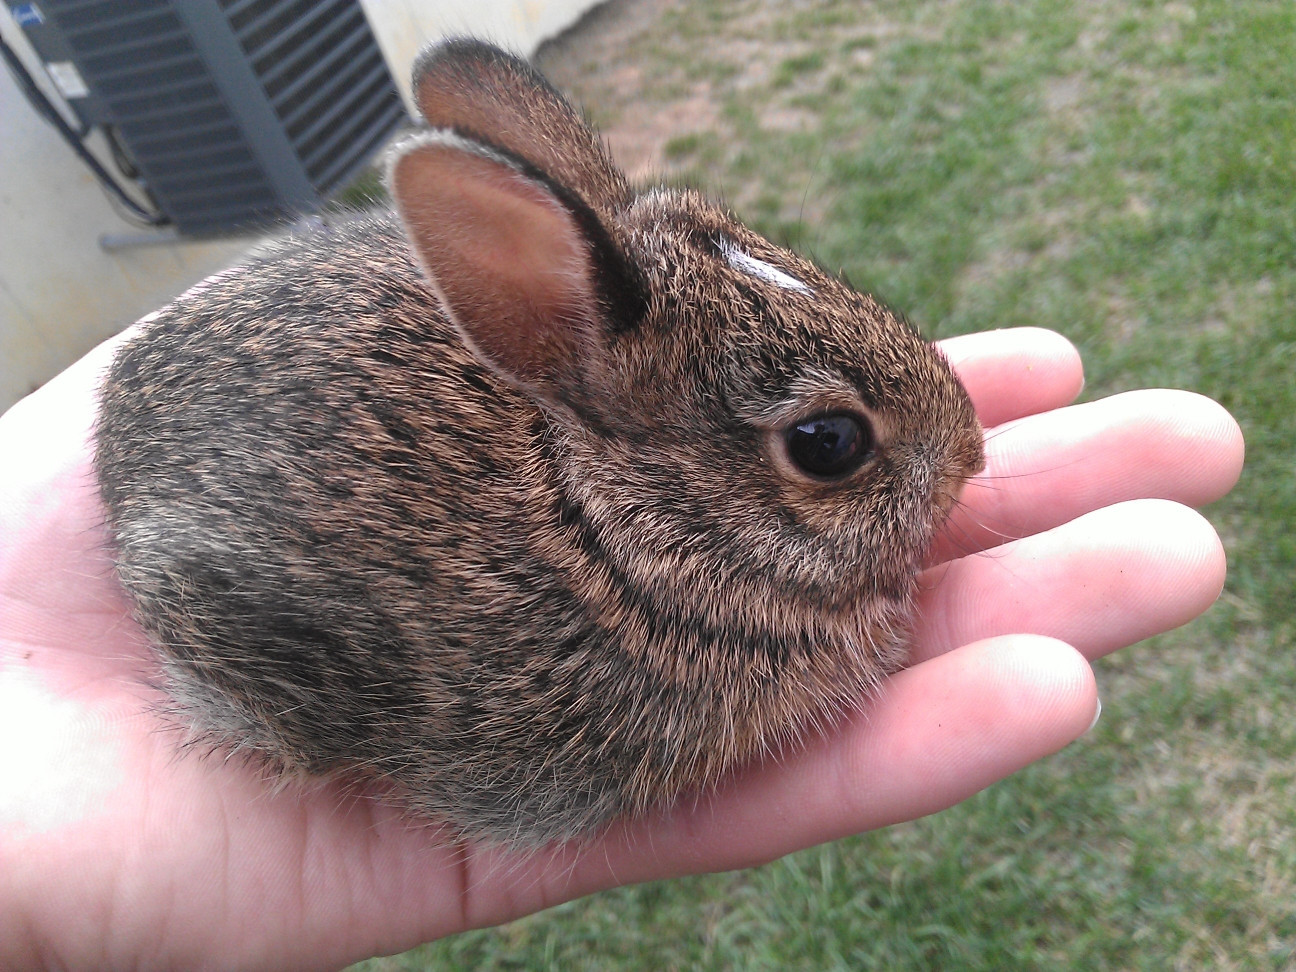
\includegraphics[width=0.7\textwidth]{img/final.jpg}
  \end{center}
\end{frame}

\end{document}
